\chapter{Computer Arithmetic and Computational Errors}

\section{Numerical Stability}

There is only finite space in computer. How would we store \( \pi \), an irrational number? We can't. We can only store an approximation of \( \pi \). How does introduction of approximations affect the accuracy of our computations?

\begin{example}
    Suppose we want to compute the value for the sequence of integrals \[
        y_n = \int_0^1 \frac{x^n}{x + 5} \, dx
    \] for \( n = 0, 1, 2, \ldots, 8 \), with 3 decimal digits of accuracy.

    There are several properties that I can claim:

    \begin{itemize}
        \item \( y_n > 0 \) for all \( n \), since the integrand \( \frac{x^n}{x + 5} > 0 \) for all \( x \in (0, 1) \).
        \item \( y_{n+1} < y_n \) for all \( n \), since the integrand \( \frac{x^{n+1}}{x + 5}
              = x \cdot \frac{x^n}{x + 5} < \frac{x^n}{x + 5} \) for all \( x \in (0, 1) \).
    \end{itemize}

    There is not closed-form solution to this problem.

    \begin{align*}
        x^n
         & = x^n \cdot \frac{x + 5}{x + 5}
         & \text{for } x \in (0, 1)                                                  \\
        x^n
         & = \frac{x^{n+1}}{x + 5} + \frac{5x^n}{x + 5}                              \\
        \int_0^1 x^n \,dx
         & = \int_0^1 \frac{x^{n+1}}{x + 5} \,dx + 5 \int_0^1 \frac{x^n}{x + 5} \,dx \\
        \frac{1}{n + 1} x^{n+1} \Big|_0^1
         & = y_{n+1} + 5 y_n                                                         \\
        y_{n+1}
         & = \frac{1}{n + 1} - 5 y_n
    \end{align*}

    Fortunately, \begin{align*}
        y_0
         & = \int_0^1 \frac{1}{x + 5} \,dx \\
         & = \ln (x + 5) \Big|_0^1         \\
         & = \ln 6 - \ln 5                 \\
         & = \ln \frac{6}{5}
        \doteq 0.182
    \end{align*}

    By the recurrence, \begin{align*}
        y_1 & = \frac{1}{1} - 5 y_0 \doteq 1 - 5 (0.182) = 0.0900      \\
        y_2 & = \frac{1}{2} - 5 y_1 \doteq 0.5 - 5 (0.0900) = 0.0500   \\
        y_3 & = \frac{1}{3} - 5 y_2 \doteq 0.333 - 5 (0.0500) = 0.0830 \\
        y_4 & = \frac{1}{4} - 5 y_3 \doteq 0.25 - 5 (0.0830) = -0.165
    \end{align*}

    Clearly, something went wrong. We have a negative value for \( y_4 \), which is impossible. We also have \( y_3 > y_2 \). The problem is that we are using floating point arithmetic, which is not exact. We are losing precision in our calculations.

    What if we leave \( y_0 \) as an unevaluated term?

    \begin{align*}
        y_1 & = 1 - 5y_0                  \\
        y_2 & = \frac{1}{2} - 5y_1        \\
            & = -\frac{9}{2} + 25y_0      \\
        y_3 & = \frac{1}{3} - 5y_2        \\
            & = \frac{137}{6} - 125y_0    \\
        y_4 & = \frac{1}{4} - 5y_3        \\
            & = -\frac{1367}{12} + 625y_0
    \end{align*}

    We approximated \( y_0 = \ln \frac{6}{5} \approx 0.182 \). We know that the true value of \( y_0 \in [0.1815, 0.1825] \). Another way to express \( y_0 \) is \( y_0 = 0.182 + E \), where \( | E | \leq 0.0005 = 5 \times 10^{-4} \) is the error in our approximation.

    Substituting this into the formula for \( y_4 \), we get \begin{align*}
        y_4 & = -\frac{1367}{12} + 625(0.182 + E) \\
            & = -113.91\dot{6} + 113.75 + 625E    \\
            & = -0.1\dot{6} + 625E
    \end{align*}
    where \[
        625 E \leq 625 \times 5 \times 10^{-4} = 0.3125
    \] and \[
        y_4 < y_0 \doteq 0.182
    \] so our propagated error is greater than the quantity to compute.
\end{example}

A lesson learned from the previous example is that the math textbook algorithms does not necessarily produce good computational algorithms. This algorithms for computing \( y_n \) is said to be an \term{numerically unstable algorithm}, since a small error was magnified by the algorithm. We want the algorithms to be \term{numerically stable}.

\begin{definition}[Numerically Unstable]\index{Numerically Unstable}
    An algorithm is said to be \term{numerically unstable} if the error in the output is not bounded by the error in the input.
\end{definition}

\begin{remark}
    In the previous example, a small error \( E \) is magnified by \( 5 \) each step.
\end{remark}

\begin{example}[Cont.]
    We can re-arrange the recurrent relation
    \begin{align*}
        y_{n+1}
         & = \frac{1}{n-1} - 5y_n                               \\
        5y_n
         & = \frac{1}{n+1} - y_{n+1}                            \\
        y_{n+1}
         & = \frac{1}{5} \left( \frac{1}{n+1} - y_{n+1} \right) \\
    \end{align*}

    We have bounded the error in the output by the error in the input, but we are at a disadvantage since we are computing backwards. How can we start this recurrent relation?

    Recall that \[
        y_{100} < y_{99} < \cdots < y_0 \doteq 0.182
    \]

    We start by approximating \( y_{100} \doteq 0 \). We know the exact value is \( y_{100} = 0 + \varepsilon \), where \( 0 < \epsilon < 0.182 \).

    Then,
    \begin{minipage}[t]{0.45\linewidth}
        \begin{align*}
            y_{99}
             & = \frac{1}{5} \left( \frac{1}{100} - y_{100} \right)            \\
             & = \frac{1}{5} \left( \frac{1}{100} - (0 + \varepsilon ) \right) \\
             & = \frac{1}{500} - \frac{\varepsilon}{5}
        \end{align*}
    \end{minipage}
    \begin{minipage}[t]{0.45\linewidth}
        \begin{align*}
            y_{98}
             & = \frac{1}{5} \left( \frac{1}{100} - y_{99} \right)                                              \\
             & = \frac{1}{5} \left( \frac{1}{100} - \left(\frac{1}{500} + \frac{\varepsilon}{5} \right) \right) \\
             & = \cdots + \frac{\varepsilon}{25}
        \end{align*}
    \end{minipage}

    {~~~}

    {~~~}

    We observe that the effect of the error is \( \varepsilon \) is diminished by a factor of \( \frac{1}{5} \) each step. This is a numerically stable algorithm. By the time we get to \( y_8 \), we can expect an accurate result.
\end{example}

\begin{definition}[Numerical Stability]\index{Numerical Stability}
    An algorithm is said to be \term{numerically stable} if the error in the output is bounded by the error in the input.
\end{definition}

\section{Floating Point Arithmetic}

\subsection{Floating Point Representation}

We only have finite space in the computer. This means we cannot store all real numbers, only an approximation of them. We use the \term{floating point representation} to store real numbers.

\begin{definition}[Floating Point Representation]\index{Floating Point Representation}\index{Floating Point!Significant}\index{Floating Point!Mantissa}\index{Floating Point!Base}\index{Floating Point!Exponent}
    A real number \( x \) is represented in the form \[
        fl(x) = \pm d_0 . d_1 d_2 \dots d_{p-1} \times \beta^e \qquad d_0 \neq 0
    \] where \( m \) is the \term{significant} or \term{mantissa}, \( \beta \) is the \term{base}, and \( e \) is the \term{exponent}.
\end{definition}

\begin{note}
    \begin{itemize}
        \item \( d_i \)'s are bounded by \[
                  0 \leq d_i < \beta.
              \]

        \item \( p \) is the precision of the accuracy.

        \item \( E \) is also bounded by \[
                  L \leq E \leq U
              \]
    \end{itemize}
\end{note}

With the floating point representation, we have a finite set of floating point numbers \[
    F(\beta, p, L, U) = \{ \pm d_0 . d_1 d_2 \dots d_{p-1} \times \beta^E : 0 \leq d_i < \beta, L \leq E \leq U \}.
\]

\begin{remark}[\( d_0 \neq 0 \)]
    We observe that this representation is not unique. Consider a system \[
        F(\beta=10, p=5, L=-10, U=10)
    \] and the number \( 1.23 \), we have the representation \[
        + 1.2300 \times 10^0 \in F(10, 5, -10, 10)
    \] but also \[
        + 0.1230 \times 10^1 \in F(10, 5, -10, 10)
    \] and \[
        + 0.0123 \times 10^2 \in F(10, 5, -10, 10)
    \]

    Thus, we need to choose a unique representation for each number. We can add a rule that \textbf{the first digit is not zero}, which normalizes the floating point representation, and makes representations unique.
\end{remark}

\begin{remark}[Representating Zero]
    Since \( d_0 \neq 0 \), how can we represent zero? We define another rule \[
        fl(0) = 0.000\dots0 \times \beta^{L-1}
    \] where \textbf{an exponent of \( L-1 \) is used to indicate the value is denormalized}.
\end{remark}

In the early days of computing, different manufacturers used different floating point representations. This made it difficult to write portable code. The IEEE 754 standard \cite{8766229} was introduced to standardize floating point representations.

\begin{table}[H]
    \centering
    \begin{tabular}{ccc}
                    & Single Precision & Double Precision \\
        \( \beta \) & 2                & 2                \\
        \( p \)     & 24               & 53               \\
        \( L \)     & -126             & -1022            \\
        \( U \)     & 127              & 1023
    \end{tabular}
\end{table}

\begin{note}
    For single precision, we have \[
        E \in \{ -126, -125, \ldots, 127 \}
    \] with a cardinality of \( 254 \). If we use \( 8 \) bits to represent the exponent, we have \( 2^8 = 256 \) possible values. We have \( 2 \) special values: \( E = L - 1 = -127 \) for denormalized numbers, and \( E = U + 1 = 128 \) for infinity and NaN (Not a Number).
\end{note}

\begin{remark}[Memory Requirements]
    For single precision, we need \( 1 + 24 + 8 = 33 \) bits to represent a number. This is a very weird number of bits. We don't know any computer that uses 33 bits to represent a number.

        {~~~}

    Turns out we only need \( 23 \) bits for the significant, since the first digit in a normalized system is always 1. We can drop the first digit, and use \( 23 \) bits for the significant, \( 8 \) bits for the exponent, and \( 1 \) bit for the sign. This gives us \( 32 \) bits, which is a more common number of bits.
\end{remark}

\begin{note}[Types in Different Languages]
    \begin{table}[H]
        \centering
        \begin{tabular}{rcc}
                   & Single Precision & Double Precision \\
            C      & \texttt{float}   & \texttt{double}  \\
            Python &                  & \texttt{float}   \\
            Rust   & \texttt{f32}     & \texttt{f64}
        \end{tabular}
    \end{table}
\end{note}

\begin{note}[Extended Precision and Reduced Precision]
    For accurate engineering, we may need more precision, called \term{extended precision} (Quad Precision). This is not part of the IEEE 754 standard, but is available in some systems.

        {~~~}

    In machine learning systems, we want the opposite -- we want to use less precision to save memory and computation time. This is called \term{reduced precision}, and we often use \( 16 \) or \( 8 \) bits. This is a topic of active discussion, and the IEEE committee is working on a standard for reduced precision for ML.
\end{note}

Note that the distribution of floating point numbers is not uniform. There are more floating point numbers near zero than near \( \pm \infty \). This is because the exponent is distributed uniformly, but the significant is not.

\begin{figure}[H]
    \centering
    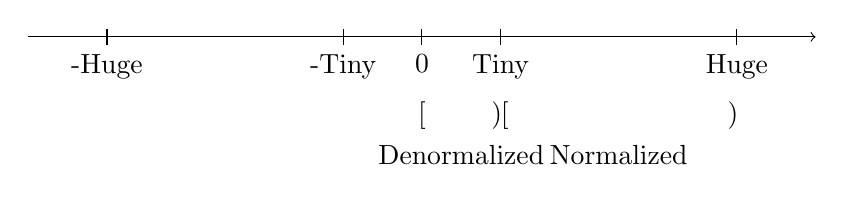
\begin{tikzpicture}
        \draw[->] (-5, 0) -- (5, 0) node[right] {\(\R\)};

        \draw (0, 0.1) -- (0, -0.1) node[below] {0};
        \draw (-4, 0.1) -- (-4, -0.1) node[below] {-Huge};
        \draw (-1, 0.1) -- (-1, -0.1) node[below] {-Tiny};
        \draw (1, 0.1) -- (1, -0.1) node[below] {Tiny};
        \draw (4, 0.1) -- (4, -0.1) node[below] {Huge};

        \node at (0, -1) {[};
        \node at (0.95, -1) {)};
        \node at (1.05, -1) {[};
        \node at (3.95, -1) {)};

        \node at (0.5, -1.5) {Denormalized};
        \node at (2.5, -1.5) {Normalized};
    \end{tikzpicture}
\end{figure}

\begin{table}[H]
    \centering
    \begin{tabular}{ccc}
         & Single
         & Double                                                          \\
        HUGE
         & \( +1.11\dots1 \times 2^{127}   \approx 3.4 \times 10^{38} \)
         & \( +1.11\dots1 \times 2^{1023}  \approx 1.8 \times 10^{308} \)  \\
        TINY
         & \( +1.00\dots0 \times 2^{-126}  \approx 1.2 \times 10^{-38} \)
         & \( +1.00\dots0 \times 2^{-1022} \approx 2.2 \times 10^{-308} \)
    \end{tabular}
\end{table}

\begin{remark}
    What about \( x \in \R \), \( x > \text{HUGE} \)? In this case, we have an overflow, and the computer will return \( fl(x) = +\infty = 1.00\dots0 \times \beta^{u+1} \).
\end{remark}

\begin{remark}
    What happens if we have \( (+ \infty) - (+ \infty) \)? In this case, we have an indeterminate form, and the computer will return \( NaN \) (Not a Number), \[
        1.xx\dots x \times \beta^{u+1}
    \] where at least one of the \( x \)'s is not zero.
\end{remark}

\begin{remark}
    For \( 0 \leq x \leq \text{TINY} \), take \[
        fl(x) = \begin{cases}
            0.00d_id_{i+1}\dots d_{p-1} \times \beta^{L-1} \\
            0 & \text{eventually}
        \end{cases}
    \]
\end{remark}

\begin{example}
    Suppose we have \[
        F(\beta, p, L, U ) = F(10, 3, -10, 10)
    \] and \[
        x = 3.00 \times 10^5, y = 3.00 \times 10^5, \qquad x, y \in \R
    \]

    Computing \[
        z = x^2 + y^2
    \] would give \[
        z = 1.60 \times 10^{11} + 9.00 \times 10^{10} \notin F(10, 3, -10, 10)
    \] and hence \( fl(z) = +\text{Inf} \).

    What if we instead want to compute \[
        z = \sqrt{x^2 + y^2}?
    \]
    Using the standard algorithm, we get +Inf inside the square root, and the computer will return NaN. We need to repair our algorithm.
    \begin{align*}
        h & = \max(|x|, |y|) \times \sqrt{1 + \left(\frac{\min(|x|, |y|)}{\max(|x|, |y|)} \right)^2}
    \end{align*}
\end{example}

\begin{remark}
    The \texttt{libm} library in C and the \texttt{math} module in python both have a function called \texttt{hypot} that computes the Euclidean distance. This is a numerically stable algorithm that avoids overflow and underflow.
\end{remark}

\begin{note}[Inf Could Have Meanings]
    Suppose you are computing the slope of a line, and you get infinity. This would indicate that the line is parallel to the y-axis. This is a meaningful result, and not an error.
\end{note}

\begin{note}[Sometimes, Underflow is OK]
    % Let \( x \in \R \), \( 0 < x < \text{TINY} \).

    % We have \( fl(x) = 0 \), an underflow, but that's OK.

    Recall the McLaurin series for \[
        y = 1 + x + \frac{x^2}{2}
    \]

    Suppose we are computing in \( F(10, 3, -10, 10) \). \[
        y = 1.00 \times 10^0 + 1.00 \times 10^{-5} + 5.00 \times 10^{-11}
    \] The last term would underflow, but that's OK. We can ignore it, since it is negligible.
\end{note}

\section{Computational Errors}

\subsection{Intuition}

\begin{example}
    We know that \( \sqrt{255} = 15.9687194227\dots \), but how should we represent this in our floating point system \( F(\beta, p, L, U) = F(10, 3, -10, 10) \)?

    The easiest solution is \term{chopping} / \term{truncation}, where we only keep the first \( p \) digits. This gives us \[
        fl(\sqrt{255}) = 1.59 \times 10^1
    \]

    Another approach is \term{round to nearest}, which gives us \[
        fl(\sqrt{255}) = 1.60 \times 10^1
    \]
\end{example}

\begin{remark}
    Heath called \( x \in \R \to fl(x) \in F \) \term{rounding}. This is why we use \term{round-to-nearest} to disambiguate.
\end{remark}

\begin{note}
    We can also round to \( +\text{Inf} \) or to \( -\text{Inf} \)
\end{note}

\begin{note}[Banker's Rounding]
    Banker's rounding is a method of rounding that rounds the last digit to the nearest even number, if it is exactly halfway between two numbers. This is the default rounding method in IEEE 754. This method is also known as \term{round to even}.
\end{note}

\begin{example}[Cont.]
    After rounding, we have error \[
        fl(\sqrt{255}) -\sqrt{255} \doteq \begin{cases}
            -0.0687 & \text{chop}             \\
            0.0313  & \text{round-to-nearest}
        \end{cases}
    \]
\end{example}

\begin{definition}[Absolute and Relative Error]
    If \( \tilde{x} \) is an approximation to \( x \), the \term{absolute error in the approximation} is \[
        | \tilde{x} - x |
    \] and the \term{relative error} is \[
        \frac{| \tilde{x} - x |}{|x|} \qquad x \neq 0
    \]
\end{definition}

\begin{example}
    The relative error of the approximation of \( \sqrt{255} \) is \[
        \doteq \begin{cases}
            4.3 \times 10^{-3}  & \text{chop}             \\
            1.96 \times 10^{-3} & \text{round-to-nearest}
        \end{cases}
    \]
\end{example}

\begin{remark}
    Absolute error is not sensitive to scale, while relative error is.
\end{remark}

\begin{example}
    Let \( x, y \in \R \), and they are approximated by \( \tilde{x}, \tilde{y} \in F \).

    Consider \( x = 100.001, y = 0.112, \tilde{x} = 100., \tilde{y} = 0.113 \). The absolute error is \[
        | \tilde{x} - x | = 0.001, \quad | \tilde{y} - y | = 0.001
    \]
    They absolute errors are the same, but this does not meas the two approximations are equally good. The relative error is \[
        \frac{| \tilde{x} - x |}{|x|} \doteq 1.0 \times 10^{-5}, \quad \frac{| \tilde{y} - y |}{|y|} \doteq 9.0
    \] The relative error for \( y \) is much larger than for \( x \), so the approximation for \( y \) is worse.
\end{example}

\subsection{Machine Epsilon}

If \( x \in \R \) is approximated by \( fl(x) \in F \), how large can the relative error be?

\begin{example}
    Consider \( F(10, 3, L, U ), a \in \R \) with \( a = w.xyz \times 10^E \) with \( 0 < w \leq 9 \),  \( 0 \leq x, y, z \leq 9 \), and \( L \leq E \leq U \).

    Assume we determine \( fl(a) \) using round to nearest, \[
        | fl(a) - a | \leq 0.005 \times 10^E
    \]

    The maximum relative error is \begin{align*}
        \max \frac{| fl(a) - a |}{|a|}
         & \leq \frac{\max | fl(a) - a |}{\min | a |}    \\
         & = \frac{0.005 \times 10^E}{1.000 \times 10^E} \\
         & = 0.005 = \frac{1}{2} \times 10^{-2}
    \end{align*}
\end{example}

In general, for \( x \in \R \) and \( fl(x) \in F(\beta, p, L, U) \) with round to nearest, we have \[
    \frac{|fl(x) - x|}{|x|} \leq \frac{1}{2} \times \beta^{1-p}
\] assuming \( x \) is representable.

This quantity is called the \term{relative round-off error bound}.

\begin{definition}[Machine Epsilon]\index{Machine Epsilon}\index{Relative Round-off Error Bound}
    The \term{round-off error bound} or \term{machine epsilon} is the maximum relative error that can occur when approximating a number, \[
        \varepsilon_{\text{machine}} = \frac{1}{2} \times \beta^{1-p}
    \]
\end{definition}

\begin{remark}
    In IEEE 754, we have \[
        \varepsilon_{\text{machine}} = \begin{cases}
            2^{-24} \doteq 5.96 \times 10^{-8} & \text{Single Precision} \\
            2^{-53} \doteq 1.1 \times 10^{-16} & \text{Double Precision}
        \end{cases}
    \]
\end{remark}

\begin{example}
    Suppose we have \( F(10,3, -10, 10) \), \( x = 1.51 \times 10^8 \), and \( y = 3.71 \times 10^6 \) , \( x, y \in \R \), \( fl(x) = x, fl(y) = y \).

    We want to compute \( z = x + y \). We have \[
        z = 1.51 \times 10^8 + 3.71 \times 10^6 = 1.5471 \times 10^8 \notin F
    \] and \( fl(z) = 1.55 \times 10^8 \).
\end{example}

\begin{remark}
    Mathematically, addition is not closed in \( F \).
\end{remark}